\scanpage{22}
b) $n$ impair $\geq1$, la suite exacte se réduit :
\[
0\longrightarrow H^n(U^n)\text{---}H^{n-1}(Q^{n-1})(-1)\text{---}H^{n+1}(Q^n)\text{---}0
\]
i.e. $H^{n-1}(Q^{n-1})$ est une extension de $H^{n+1}(Q^n)$ par

a) Cohomologie de $Q^n$ nulle en dim impaire.

b) $H^i(U^n)$ nul si $i\neq0,n$, isomorphe à $A$ (resp. $A\otimes V_n$) si
\figure{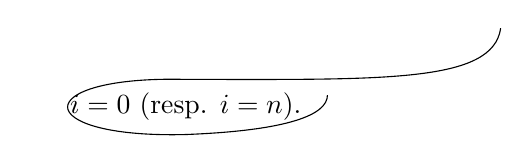
\begin{tikzpicture}
\node at (0,0) {$i=0$ (resp. $i=n$).};
\draw (4,1) .. controls (3.9,.3) and (2.5,.35) .. (0,.35) .. controls (-2,.4) and (-2,-.4) .. (0,-.35) .. controls (1.3,-.3) and (1.8,-.1) .. (1.8,.15);
\end{tikzpicture}}

b') Énoncé dual

c) $H^{\unsure{i-2}}(Q^{n-1})(-1)\longrightarrow H^i(Q^n)$ est
\[
\left|\begin{array}{l}
\left.\begin{array}{l}
\text{bijectif si }\deleted{\unsure{i\neq0,2}}\inserted{i\geq2},\ i\neq n\\
\text{injectif pour tt }i
\end{array}\right\}(n\text{ \uline{pair}})\\[2pt]
\left.\begin{array}{l}
\text{bijectif si }i\geq2,\ i\neq n+1\\
\text{surjectif pour tt }i\geq1
\end{array}\right\}(n\text{ impair})
\end{array}\right.
\]
\unsure{d'|c'}) Énoncé dual: $H^i(Q^n)\longrightarrow H^i(Q^{n-1})$ est
\[
\left|\begin{array}{l}
\left.\begin{array}{l}
\text{bijectif si }i\leq2n-2,\ i\neq n\\
\text{surjectif pour tt}
\end{array}\right\}n\text{ \uline{pair}}\\
\left.\begin{array}{l}
\text{bijectif si }i\leq2n-2,\ i\neq n-1\\
\text{injectif pour tt }i\leq2n-1
\end{array}\right\}n\text{ impair}
\end{array}\right.
\]
d) $H^{\unsure{i|2i}}(Q^n)$ \deleted{de rang} est de rang $1$ en toute dimension \inserted{paire} \uline{sauf} pour $n$ pair et \deleted{\unsure{2}} $i=n$, où il est de rang $2$.

e) Si $n$ pair,

\margin{
\diagram{\begin{tikzcd}[column sep=large,row sep=large]
\unsure{F}\\
X\arrow[dr,no head]\arrow[r,phantom,"\subset" description]&X'=Y[\unsure{h,-1_h|h,1/h}]\arrow[d,no head]\\
&Y
\end{tikzcd}}
}
\mspage{21}
